% !% !TeX spellcheck = en_GB
\chapter{The Chinese sword}\label{ch:chinesesword}

Broadly, a sword can be defined as a cutting and thrusting edged weapon with a blade at least as long as the arm and a short handle.

There is archaeological evidence of the use of swords dating back as far as the Bronze Age, both in the Occidental world and in China.

From these early times to the beginning of the XX\textsuperscript{th} century when they ceased to be used for combat, swords have evolved in parallel with fighting techniques and strategies.
The swordsmanship of any particular historical period was adapted to the currently available types of swords while being at the same time deeply rooted in its social and cultural context.

Thus, \Taijijian{} adopted the kind of straight double-edge swords, or \Jian{}, that were being commonly used at the time by every Chinese martial art.
Although there had never been in historical times any sword specifically tailored for the practice of \Taijijian{}, this Chinese double-edged sword is nowadays often abusively denoted by the term \Taiji{} sword.

\section{From the battlefield to the public park}
I will not get deep into historical considerations about Chinese swordsmanship. Others, more knowledgeable on the subject than I am, have already published works more accurate and extensive than anything I could write here.
For a more detailed account, I can only refer the interested reader to Peter Lorge's book \textit{Chinese Martial Arts: from Antiquity to the Twenty-First Century} and Scott Rodell's \textit{Chinese Swordsmanship}.

After having dominated Chinese battlefields until the late XIX\textsuperscript{th} and early XX\textsuperscript{th} century, edged weapons were eventually superseded by modern firearms and artillery. Practical sword fencing rapidly declined during the early XX\textsuperscript{th} century.
\ChenWeiming{}, in his book \textit{Taiji sword}, first published in 1928, mentions fencing only to say that \YangChengfu{} never taught any sword fencing set, and that he would himself write another sword book when he becomes proficient in it. As far as I can tell, this book was never written.
During the 1930s and 1940s, Chinese sword manuals lament that this ancient art was almost completely lost. 

At the same period, as China was falling under the influence of Western Empires, invaded by Japanese troops, then ravaged by the Civil War, Chinese martial arts were becoming symbols of national pride while gradually turning into disciplines for physical education, health and self cultivation.

Boxing and wrestling soon overtook weapon training, which was reduced to a mere form practice and a complement to unarmed martial arts. 
The primary goal of Chinese martial arts instructors was not to train combatants any more, but to strengthen their nation by invigorating their fellow compatriots while expressing the superiority of Chinese tradition.
Practical fencing was not sought, but swift and athletic demonstrative movements started to be favoured over effectiveness in combat.
Light swords with extremely flexible blades were more and more commonly used and somewhat became the norm.

Though there is to my knowledge no written mention of a martial art called \Taijiquan{} before the XIX\textsuperscript{th} century, the \Taiji{} principles had certainly been around for quite a long time when they were gathered into a whole coherent martial system, supposedly by the \Chen{} family of \Chenjiagou{}, and later formalised by scholars in the texts we know today as the \Taiji{} Classics.

The general \QiJiguang{} (1527\textendash{}1587), as early as the XVI\textsuperscript{th} century, cites in his \textit{New Manual on Military Efficiency} technique names that should sound familiar to every \Taijiquan{} practitioner.
It is unclear, however, whether \QiJiguang{} was actually writing about \Taijiquan{}, or its ancestor, or whether it was a mere coincidence or a later reuse of technique names.

In any case, it is generally admitted that \Taijiquan{} emerged and developed between late XVII\textsuperscript{th} and the  XIX\textsuperscript{th} century, during the \Ming{} and \Qing{} dynasties.

The \Yangjia{} \Michuan{} style, root of the present work, was created by \Yang{} \Luchan{}, presumably during the first half of the XIX\textsuperscript{th} century.
I have no clear evidence that the \Yangjia{} \Michuan{} \Kunlun{} sword form originates from this period, but the rhymes that describe the movements seem to point to a rather ancient origin.
\QiJiguang{}'s treatise contains indeed a collection of such rhymes that were used as mnemonics for routine practice.

Originally, forms had been used for training troops of soldiers to manoeuvre and fight in unison. However, as early as during the \Tang{} dynasty, training sessions shifted towards a sort of martial spectacle, not only for military power display, but also as a mere entertainment. 
In order to please spectators who often were not martial artists themselves, forms increasingly incorporated demonstrative techniques that would be much more spectacular or aesthetic than truly effective.
This interest for martial spectacles has persisted to this day in literature, Chinese Opera, cinema, and, of course, in the unavoidable demonstrations performed during Martial Arts gatherings.

Nowadays, like any other Chinese martial art, \Taijijian{} has definitely left the battlefield for the public park and sword training is fortunately anything but a preparation to combat.

Despite their undeniable aesthetic dimension, however, traditional \Taijijian{} forms were originally designed to develop martial skills based on the \Taiji{} principles, effectively using swords whose weight, dimensions and balance achieved a compromise between cutting power, thrusting precision, and swift movements.

\section{Anatomy of the \Jian{}}
The figure \ref{fig:sword_parts} shows the disassembled parts of a \Jian{}, or Chinese double-edged sword, typical of the \Ming{} and \Qing{} dynasties. 

\begin{figure}[ht]
\centering
	\includegraphics[width=0.69\textwidth]{../../Images/SwordParts/SwordPartsEn.pdf}
	\caption[Sword parts]{Sword parts: The double-edged straight blade is extended by the tang, traversing the guard, handle and pommel where it is secured by peening. The two ferrules are metallic rings preventing the extremities of the handle from splitting open. The guard protects the hand holding the sword. Usually made of bronze or a similar metal, it is hollow and open towards the front. The handle, generally made of wood, is spindle-shaped and sometimes covered with a string, leather or ray skin in order to prevent the grip from slipping.
The pommel, made of the same metal as the guard plays a crucial role in the sword's balance and behaviour by counterbalancing the weight of the blade.}
	\label{fig:sword_parts}
\end{figure}

The main particularity of the \Jian{}'s blade is its very gradual taper with nearly parallel cutting edges. From approximately 3 or \unit{4}{\centi\meter} at the base, the blade width decreases only to 2 or \unit{3}{\centi\meter} near the tip, where the edges curve rapidly into a sharp point.
With a blade length of 70 to 80 cm, the angle between both edges is hardly noticeable, in sharp contrast to the more triangular shape of many European mediaeval swords

Traditionally, the section of the blade could be either lenticular or diamond-shaped with a clearly marked central ridge.
Some blades could also have a \index{fuller}fuller, which is often wrongly called \emph{blood groove} because of the legend pretending that its role was to let the blood flow out of the wound.
Another delusion about the fuller is that it would prevent the blade from being stuck in the wound because of a supposed phenomenon of suction or a hypothetical contraction of the severed muscles.
I must say that I do have serious doubts about the capacity of a wounded muscle to contract significantly around a sharp blade without suffering any further damage. And assuming it could, there is certainly no reason why the blade could not cut its way out quite easily.

The truth is far less enthralling: a \index{fuller}fuller simply makes a lighter blade without compromising its solidity. Of course, the easiest way to reduce blade weight is to make it thinner. This, however, is limited by the resulting increase in flexibility, which might not be desirable beyond some degree. It also flattens the edge geometry, which might in turn affect edge durability. The \index{fuller}fuller permits a lighter blade without at the same time affecting flexibility and edge geometry.
For example, a fuller 1 cm wide and 2 mm deep, running along two thirds of a 75 cm blade with a lenticular section, would have a volume of approximately \unit{10}{\centi\meter\cubed}. As steel density ranges from \unit{7.3}{\kilo\gram \per \deci\meter\cubed} to \unit{7.8}{\kilo\gram \per \deci\meter\cubed} depending on its composition and heat treatment, such a fuller on each side of the blade would reduce its weight by about 150 g without affecting the profile of its edges. (see figure \ref{fig:blade_section}) 
This could certainly make a difference considering that a lighter blade would also mean lighter fittings. Thus, this fuller would allow a swordsmith to make a 900 g sword, the typical weight of a historical \Jian{}, with the same edge profile and blade length as a non-fullered sword weighing over 1 kg.

\begin{figure}[ht]
\centering
	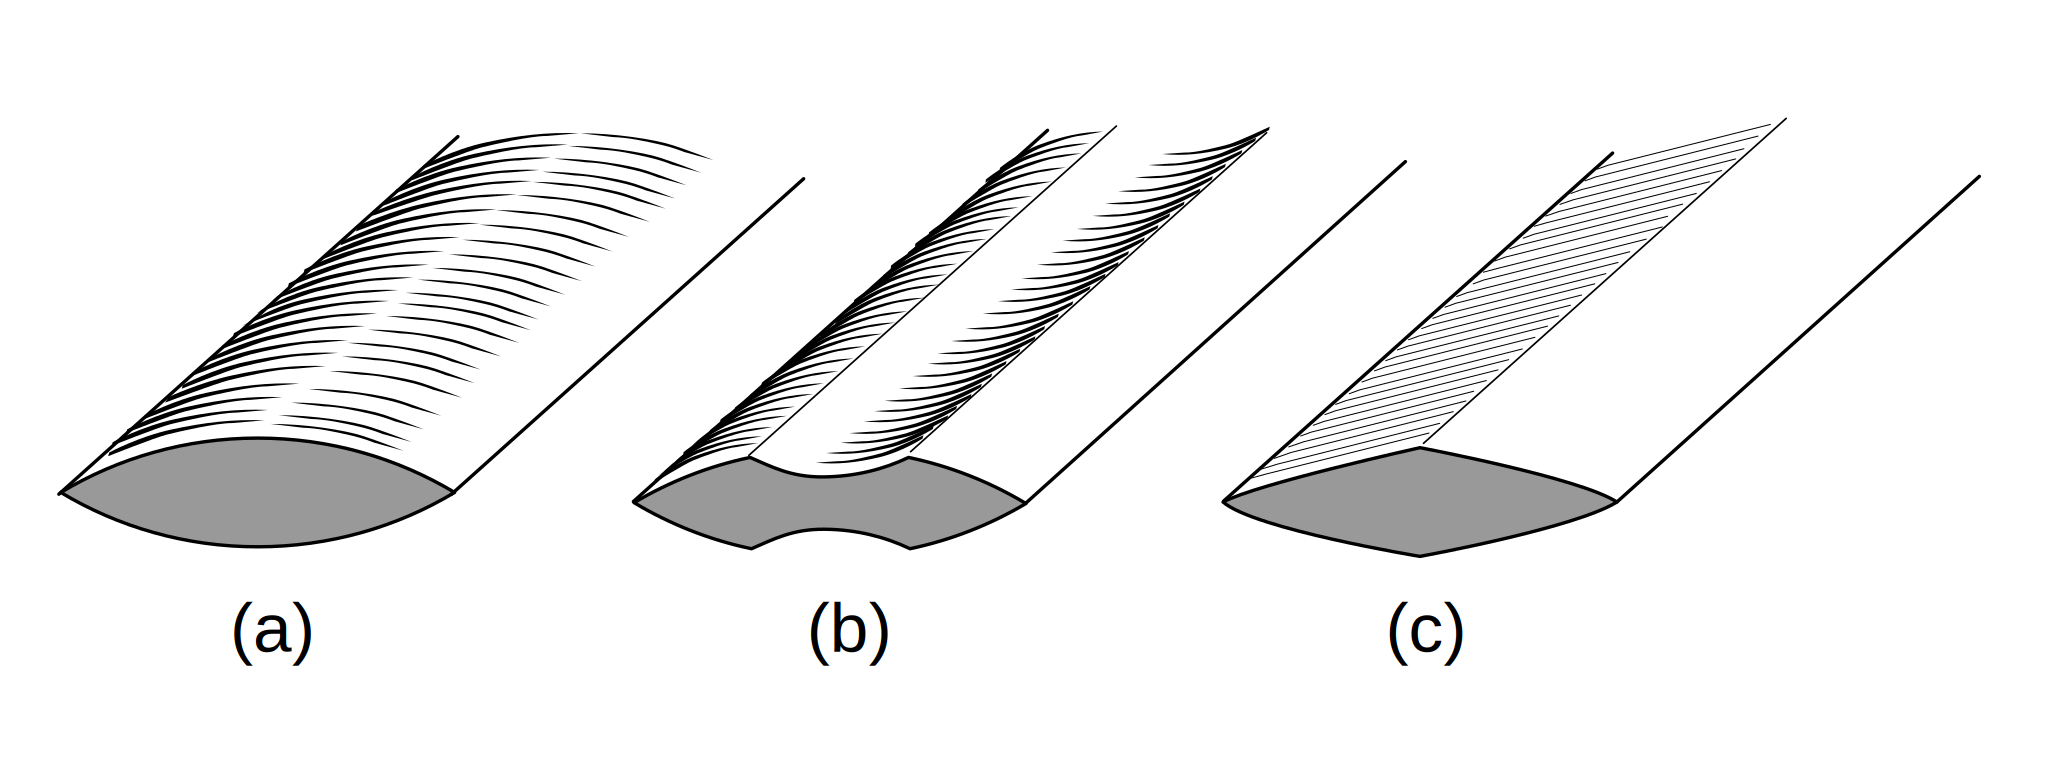
\includegraphics[width=0.69\textwidth]{../../Images/BladeSection/BladeSection.pdf}
	\caption[Blade section]{Blade sections: (a) Lenticular, or apple-seed. (b) This fullered lenticular blade has the same edge profile as the blade shown in (a), but it is significantly lighter thanks to the fuller. (c) Diamond-shaped.\\
	NB: for a clearer picture, the blade thickness has been exaggerated on this figure.}
	\label{fig:blade_section}
\end{figure}

If the blade profile may have an effect on edge durability, the kind of steel the blade is made of will also affect edge strength.  
If the steel is too soft, edges may bend and become dull after only a few cuts. Hardened steel is necessary for keeping the edges sharp, but it is also brittle and a blade cannot be made exclusively of hard steel. 
A compromise had thus to be found between blade hardness, softness and elasticity.

Note that elasticity is not a synonym for flexibility: it is the capacity of the blade to bend and return to its original shape. If the limit of elasticity is exceeded, the blade is permanently deformed or breaks. 

The blade must be hard enough for keeping its edges and at the same time sufficiently resilient and elastic so as to sustain strong blows and shocks without breaking nor taking an unwanted bend.
%Blade elasticity will also help dissipate the energy from shocks and strong blows. Vibrations, vibration node in the handle

Steel is basically a mixture of iron and a very small proportion of carbon, between 0.1\% to 2\%. It can also be alloyed with a small amount of other metals such as chromium, nickel, manganese, etc.
Even in such small quantities, these elements may, in conjunction with heat treatment, dramatically change steel mechanical properties.

\index{quenching}Quenching is a process consisting in heating the blade at a high temperature and then cooling it down rapidly by immersion into water. 
Following this treatment, steel assumes a particular crystal structure which makes it harder, but also more fragile.
Furthermore, since it is impossible to cool instantly and homogeneously the whole blade at once, quenching also creates persistent tensions in the metal that may greatly weaken the blade.
To release these constraints without reverting the hardening effect of quenching, it is possible to apply a second heat treatment, called tempering\index{tempering}. It consists in reheating the blade at a lower temperature before leaving it to cool down naturally, so as to recover sufficient resilience.

An alternative to these two successive treatments is the technique called \index{tempering!differential tempering@\textit{differential tempering}}differential tempering. Well-known for being the traditional way of Japanese swords making, this technique was originally used also in China.
In differential tempering only the edges are exposed to the quenching treatment thanks to the application of clay onto the core of the blade, which is thus protected from the heat shock and remains elastic while the edges are hardened.

In mediaeval Europe, hardened edges were sometimes welded on a soft core. As far as I know, this technique was used in China only for broad swords.
Chinese straight swords traditionally had a three-layer pattern called \SanMei{}. The blade was made of three layers of steel welded together: a thin central one of hardened steel forming the edges, and two layers of softer steel or iron protecting the former from being shattered by strong blows and providing the blade with an elastic structure.

\section{Balance and dynamic properties}\index{balance}
A sword's balance is traditionally expressed by the location of its \index{centre of gravity}centre of gravity (COG) also known as the centre of inertia. For a \Jian{}, the COG is usually located about 10 to 20 cm in front of the guard, as measured from the forward end of the handle.

But I think that there is usually too much emphasis on the COG location. Although the COG does play an important role in sword handling it is far from being the main feature affecting sword's tractability. While the COG of an object describes its static balance and how it responds to the global application of a physical force independently of its actual shape, dynamic rotational properties also depend on mass distribution and shape. This is why a rod and a ball do not handle the same at all although both have their COG located at their geometric centre.

Dynamic rotational properties are thus even more essential and determine how the sword feels when wielded, how it moves, rotates and responds to the actions exerted on the handle. As a matter of fact, it is not uncommon to find swords with a COG located at the same distance from the handle but feeling completely different when wielded. 

But measuring the physical property relating to sword rotational dynamics, the momentum of inertia, is not that easy, and even when it has been measured, interpreting this scientific value in terms of practical sword handling is far from being straightforward. 

One way of accurately measuring the momentum of inertia of a sword is the pendulum test which consists in measuring its natural oscillation period around an axis located at a given distance of the COG. After a bit of maths, you end up with a figure that will not tell you much without any reference, to be honest. More research is definitely needed here.

A much easier way to examine the dynamic properties of a sword is the waggle test. Although it is much less accurate, it has the advantage of providing some indication on how these properties actually relate to how the sword will react to your actions on the handle.

To perform this test, hold the sword lightly by the handle between your thumb and forefinger, and then wave it smoothly sideways. You will notice a point somewhere in the blade that does not move: this is the\index{pivot point} pivot point relative to the place of the handle where you were holding the sword (see figure \ref{fig:pivot_points}).

\begin{figure}[ht]
\centering
	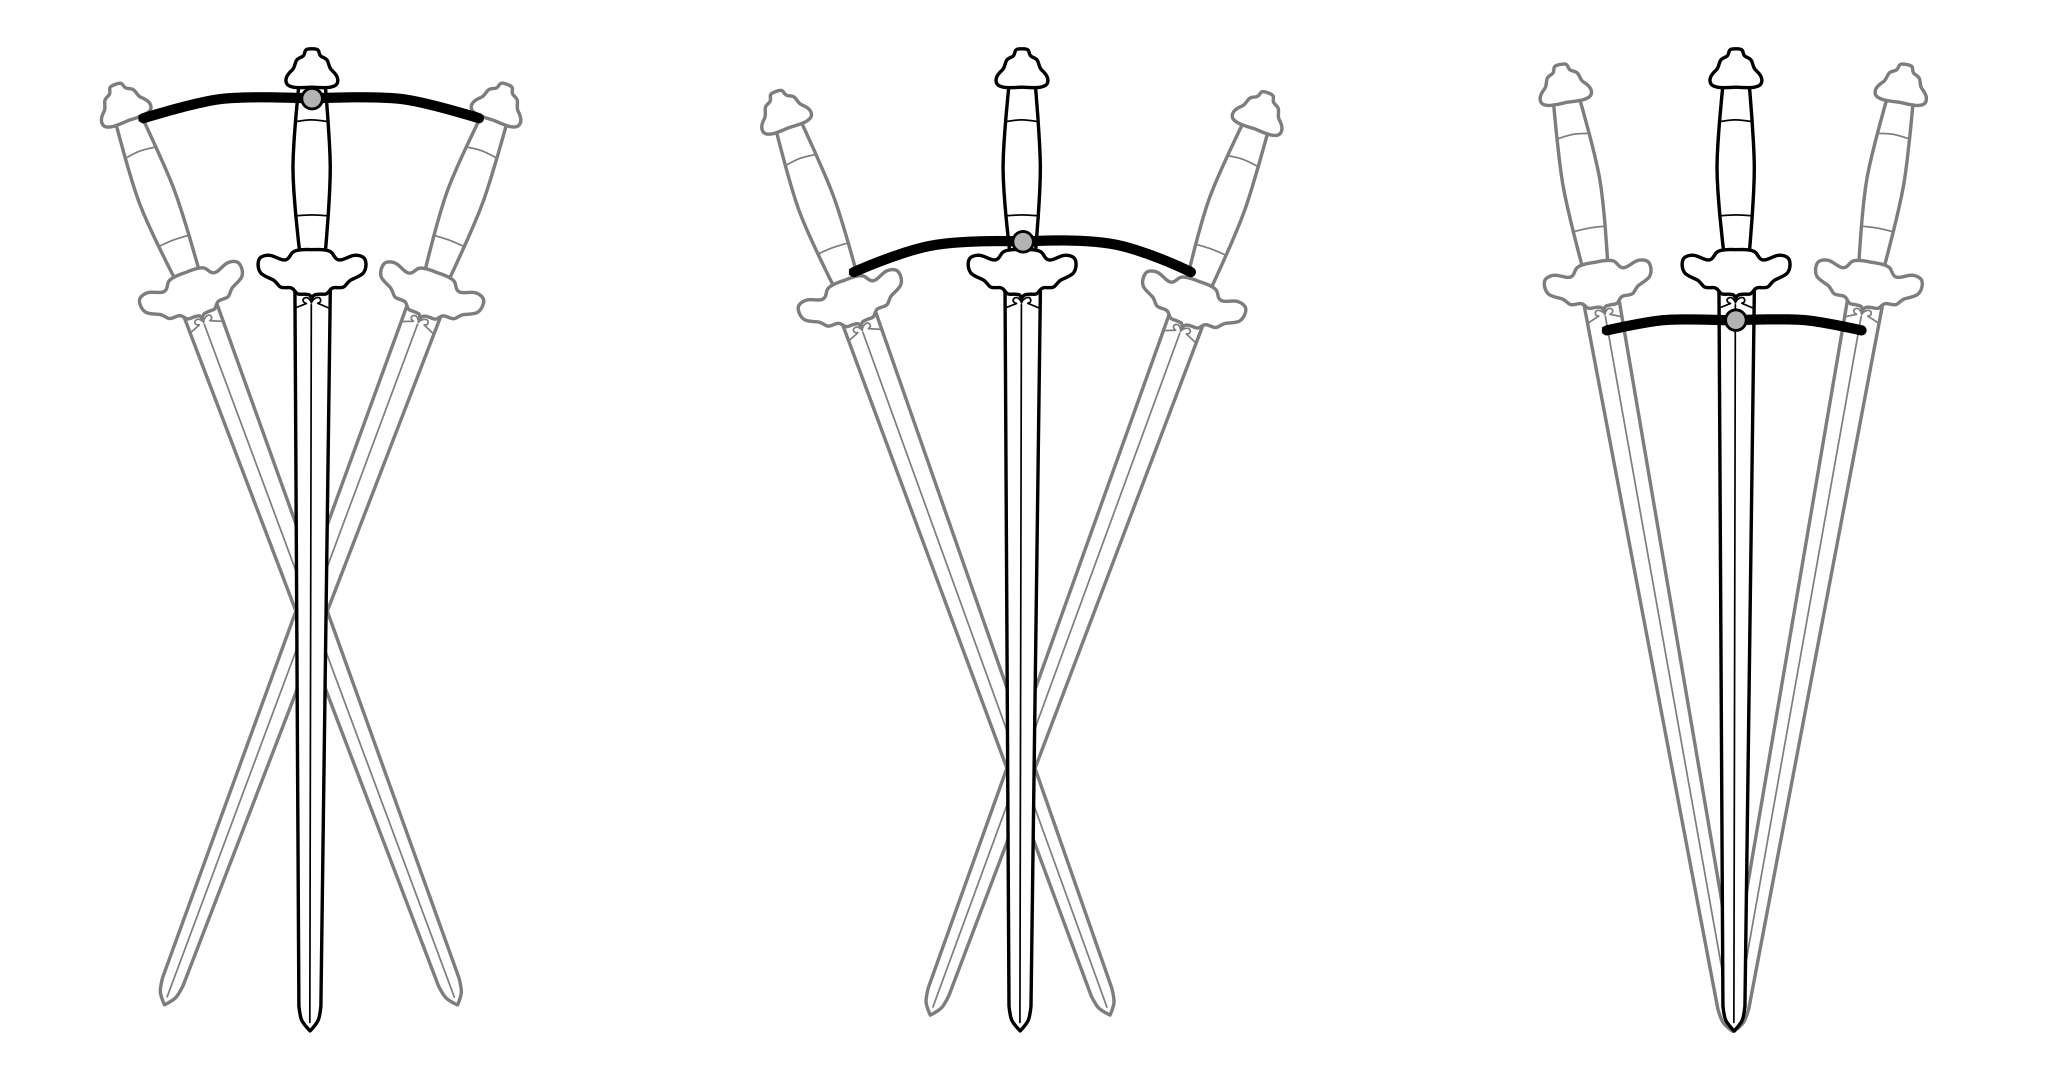
\includegraphics[width=0.80\textwidth]{../../Images/PivotPoints/PivotPoints.pdf}
	\caption[Pivot points]{A pivot point is the natural centre of rotation of the sword relative to the place and direction of an action applied to the handle. If the sword is held near the pommel and waved sideways, the pivot point is close to the centre of the blade (left). Holding the sword close to the guard will move the pivot point further down the blade towards the tip (middle). To place the pivot point at the tip of the blade for this sword, a lateral action must be applied about an inch in front of the guard (right). Although this may seem an inconvenience, a proper adjustment of the grip and a slanted action on the handle nonetheless allows the control of this point. Furthermore, this may also help to keep the blade tip in line when thrusting while controlling the opponent's blade with the guard.}
	\label{fig:pivot_points}
\end{figure}

Changing the position of the fingers on the handle will move the pivot point to another location. When wielding a sword, it is thus possible to control the location of the sword's centre of rotation by adjusting the place and direction of the action applied by the grip on the handle.

The pivot points relative to the hilt, are usually located within the first half of the sword's length starting from the tip. 
Their location is determined by the mass distribution along the sword and in particular by the relative masses on each side of the grip. Factors affecting this distribution in an unmounted blade are the form and dimensions of its cross section, how it tapers and becomes thinner towards the point, and its proportion to the tang. Adding a pommel to an unmounted blade, even a relatively light one, will dramatically modify the sword's dynamic properties, not only bringing the COG towards the hilt, but also displacing the pivot points towards the tip. However, too heavy a pommel would result in pivot points located too far forward, possibly even beyond the tip. On the contrary, too light a pommel would make it difficult or even impossible to obtain a pivot point at the tip of the blade. Achieving an appropriate range of pivot points enabling a proper control of the sword thus results from a precise blade shape design and an accurate adjustment of the blade and pommel respective weights. 

The interested reader will find more information on the subject in the book \textit{Das Schwert \textendash{} Gestalt und Gedanke/The Sword \textendash{} Form and Thought} published by the \textit{Deutches Klingen Museum} in Solingen. Although it presents exclusively western swords from different periods, this book provides a wealth of information about sword balance and dynamics equally applicable to Chinese swords. 

\section{Choosing a \Taijijian{} sword}
%\subsection{Which sword for which practice?}
There is a large variety of practice swords available on the market for \Taijijian{} and choosing one is usually much a matter of personal preference and budget.
Most of these swords, however, are only distantly related to the real weapons that were still in practical use when traditional \Taijijian{} forms were created.
Many of them have a very poor balance and are either too light or too heavy.
Whereas the actual weight of a practice sword is not that important and should be adapted to the practitioner's fitness and experience, the sword's balance and dynamic behaviour is crucial and should never be overlooked.
Security in two-person drills and free play are also an absolute priority.

Practitioners with a strong interest in all dimensions of \Taijijian{} will most certainly end up possessing at least two swords, one for form practice and the other one for partner drills and free play. 
%If, fundamentally, nearly no restriction applies to form practice, it is important for two-person drills and free play, that blades are neutralized and adapted to the protections worn by the pratitioners.

\subsection{Form practice}\index{form!choosing a sword@\textit{choosing a sword}}
As traditional form movements were adapted to the balance of historical swords, wielding such a weapon, even a quite heavy one, should have been effortless when performing the form if the \Taiji{} principles were respected. 

Nowadays, practising the form with a sword having dimensions, weight and balance similar to those of historical ones can only bring us closer to the essence of traditional sets.
Handling such a sword may well be much more demanding than using a lightweight blade, it is nonetheless an incomparable and challenging opportunity to make progress on our way towards a deeper understanding of our art and a better embodiment of the \Taiji{} principles.

However, while it is true that a heavier sword may be a better guide for form practice than a lighter one, it is also much less forgiving of technical mistakes and excess of muscular tension.
The weight of the sword should thus be adapted to the practitioner's experience and fitness. There is no point for a beginner to practise with a heavy sword that would do nothing but strain his joints and muscles at every clumsy move he would make. 
Thus, practising with a wooden or cheap light steel sword will be acceptable for an absolute beginner to memorize the form, but will soon become limiting when it comes to more in-depth practice.
Once he has gained sufficient experience, it is advisable for the practitioner to change for a well-balanced sword weighing approximately a historically accurate 700 to 900 g.

Similarly, beginners learning the form and basics may be unnecessarily hampered by a long blade and should favour shorter ones. More experienced practitioners though, if their grip is truly relaxed, should be able to easily accommodate a longer blade provided it is not extremely long.
A popular rule of thumb to determine the right length for the blade consists in holding the sword vertically along your left arm, like at the overture of the form. The tip of the blade should reach the height of your ear. Basically, this is equivalent to making sure that the blade is longer on average than the length of the arm of most opponents. They would thus not be able to protect themselves from a thrust by blocking it at the guard. 
In any case, a blade from 70 to 75 cm long should be convenient for most people. 

Whether the sword should have a \index{tassel}tassel or not depends on the style. Some use a tassel, others, like the \Yangjia{} \Michuan{}, do not.
Much has been said about the role of the tassel. It is widely accepted that, during form performance, the way the tassel is moving provides an indication of the practitioner's quality of movement. 
I am willing to accept the argument, as the tassel may be a pedagogical tool to balance the intention between the sword tip and the hilt. But if too much attention is paid to the tassel, the practitioner may well end up performing a tassel form. 
I am much less convinced by some other explanations such as the use of the tassel to distract the opponent. I personally prefer to threaten the opponent with the blade, which is much more distracting and, contrary to the tassel, is sharp and cannot be grabbed.

Actually, if we refer to historical representations of swords and swordsmen, it seems that the tassel is a rather late invention. My guess is that it was a decorative evolution of the lanyards that can be seen on earlier pictures and were used to secure the sword in the hand when fighting.
In any case, as I do not use a tassel, my only advice about it is to do whatever is recommended by the style you practise.

\subsection{Two-person drills and martial applications}\index{two-person drills!choosing a sword@\textit{choosing a sword}}\index{martial applications!choosing a sword@\textit{choosing a sword}}
Simple safely structured partner drills such as sticky swords, guiding and following, etc. might be practised with same sword as you practise the form with, as long as no attack is aimed at the face or the upper body.

I nonetheless recommend to restrict unprotected drills to well-trained experienced practitioners who are used to practise together. In all other occasions, the use of specially designed swords and appropriate protective gear \textendash{} a fencing mask and gloves at the very least \textendash{} is a necessity to limit as much as possible the risks of accident. 

Steel rigid blunt swords with a leather-covered tip are a good and relatively cheap compromise if you are on a budget. However, it should be remembered that those swords were not designed for this purpose, and they may be dangerous without the appropriate protections and precautions. Accidents may happen, and whoever uses such swords for partner work does it at their own risks. Note that I do not recommend to blunt a so-called flexible blade as they are not only unsuitable for partner work, they are also usually so thin that they are nearly sharp. 

Contrary to what is often thought, wooden swords are not really safer since, due to their stiffness, they cannot curve to absorb effectively the shock of a thrust.
Furthermore, the thickness of wooden blades hinders the feeling of blade contact which might be a problem for some kind of exercises.

The best option is definitely to use swords specifically designed for sparring. Their thick rounded edges and rolled tip will make them pretty safe provided you are wearing at least a fencing mask and padded gloves. A padded jacket may provide extra protection for more drill intensity. In addition, since they weigh over 800 g, they are less forgiving of mistakes than lighter swords when it comes to performing techniques in compliance with principles, which is an asset for technical applications and drills. 

%\begin{figure}[ht]
%\centering
%	\includegraphics[width=0.80\textwidth]{../../Images/SwordFlex/SwordFlex.pdf}
%	\caption[Blade flexibility]{The blade should be flexible enough to bend and absorb most of the energy of thrusts. A bending blade is also an indication that the distance was appropriate for the thrust: the blade curves in proportion to  how deep a wound it would have caused in a real fight.\\
%	The swords used here are Dragon Sports's upper range rigid \Taiji{} swords with a leather-covered tip. Both partners are wearing fencing masks, gloves and Axel Pettersson padded jackets.}
%	\label{fig:sword_flex}
%\end{figure}


\subsection{Free play}\index{free play!choosing a sword@\textit{choosing a sword}}
Though gentle soft games can be played with unprotected blade or blunt steel swords with a leather-covered tip, I strongly recommend to always use specifically designed swords associated to appropriate protective gear (fencing mask, padded gloves and padded fencing jacket).
Even if attacks are voluntarily restricted to the lower body, instinctive reactions may cause accidents with dramatic consequences without the appropriate equipment and precautions.

Wooden swords are not more suitable for free play than they are for partner drills. Uncontrolled vigorous cuts hitting fingers or bones are not less painful nor dangerous than with a steel sword. Contrary to steel blades, wooden swords will not bend on thrusts and all the energy of the shock will be transmitted to the target instead of being partly dissipated by the blade.

A good sword for free play should have a rounded or rolled tip and thick rounded edges for safer thrusts and cuts. It should be heavy enough to enforce correct techniques and prevent unrealistic quick wrist movements similar to those seen in western modern fencing with the foil. However, its balance should allow all the techniques found in your \Taijijian{} forms to feel natural with swift and easy transformation.

There are now Chinese steel swords designed for sparring and partner drills available on the market. My favourite model, and the one we use in our group, is produced by \textit{Péter Regenyei Armory}. This sparring \Jian{} is the result of a collaboration between Mattias Nyrell, the main \Jianfa{} instructor of \textit{Historisk Fäktning i Linköping}, the renowned swordsmith Péter Regenyei and Peter Dekker, an antiquarian founder of \textit{Mandarin Mansion} specialized in antique arms and armours from China and other regions of Asia.

This sword's design was based on a historical \Tuanlianjian{} belonging to Peter Dekker's personal collection. Those modest practical swords are also known as \textit{militia swords} since they were most certainly made for use by rural militia to defend their goods and homes. The Regenyei sparring \Jian{} design thus contrasts dramatically with the usual gilded and affected style of most Chinese swords on the market. However, in its simplicity, this sword does reflect the artisanal beauty and quality of its fabrication. 

The 73 cm long gently tapering blade has a rolled tip, flattened diamond-shaped cross section and thick rounded edges of approximately 1 to 2 mm. Those thick edges and rolled tip ensure a good dissipation of the energy when landing cuts or thrusts on protective gear. This should not be regarded though as an incentive to cut or thrust with full strength. While this blade has some degree of flexibility indeed, it nonetheless is pretty stiff and it might be a good idea to wear a chest protector, especially for women, and a throat protector in addition to the regular padded jacket. 

Despite an actual weight between 800 and 900 g, this sword feels pretty light in the hand, with a very homogenous sensation from tip to pommel. The only thing that may require to get used to is the somewhat squarish handle, but this might be an asset after all for free play as it makes it easier to feel the blade alignment when wearing padded gloves.

Its excellent balance makes a swift and nimble sword that is very easy to control provided you are properly connected and you are moving it with your body and not from your wrist or your arm only. All moves and transformations feel natural and lively, either while performing the \Yangjia{} \Michuan{} \Kunlun{} sword or when sparring.

I can only recommend the \Taijijian{} enthusiast to invest in this sword. As a matter of fact, should you own only one sword, this is the one: it is indeed perfect not only for sparring and partner work but also for form practice. 

% blade is pinned on the handle, not screwed, therefore no risk to unscrew with shocks. 
%For ensuring a good control, the sword weight should be kept on the lower end, but not too light in order to prevent unrealistic quick wrist movements, similar to those seen in western modern fencing with the foil.
%A well-balanced sword weighing about 700 g to 800 g should feel comfortable while being heavy enough to enforce the actual application of form movements.

%The blade edges should be rounded and thick enough so as to avoid cutting. Even a blunt sword can cut and split open a soft target, and protections have their limits. Since free play can be very fast and unpredictable, it remains dangerous if the intensity of the play is not adapted to both partners' experience and to the capacity of the protective gear to absorb the shocks.
%If a thick blade will probably be less prone to cutting, it nonetheless may well hurt if hurled too vigorously.






